{\color{red}*}\PID
Отпорник отпорности $R = 50\unit{\Omega}$ прикључен је на идеалан генератор простопериодичног напона облика 
$v_{\rm g}(t) = V_{\rm m} \cos(\upomega_0 t)\,\uu(t)$, где су $V_{\rm m} = 10\unit{V}$, 
$\upomega_0 = 2\uppi f$, и $f = 5\unit{Hz}$. Загревање отпорника описано је термичким 
процесом као LTI систем првог реда описан диференцијалном једначином 
$\uptau \dfrac{\de (\uptheta-\uptheta_0)}{\de t} + (\uptheta-\uptheta_0) = R_{\uptheta} p_{\rm R}$, где је 
$\uptheta = \uptheta(t)$ тренутна температура отпорника, 
$p_R = p_R(t)$ тренутна снага отпорника, параметар
$\uptau = 100\unit{ms}$ је временска константа тог термичког процеса,
 параметар $R_{\uptheta} = 20\unit{^\circ C/W}$ назива се термичком отпорношћу 
отпорника, а $\uptheta_0$ је температура амбијента. 
(а) Ако је у почетном тренутку температура отпорника једнака температури амбијента $\uptheta(0) = \uptheta_0 = 25\unit{^\circ C}$,
одредити снагу отпорника у зависности од времена, и скицирати њен график. 
(б) Израчунати амплитуду варијације температуре отпорника по успостављању 
устаљеног режима. 
\\[2mm]

\textsc{\myul{Решење:}}
Тренутна снага отпорника одређена је изразом 
$p_{R}(t) = \dfrac{v_{\rm g}^2(t)}{R} = \dfrac{V_{\rm m}^2 \cos^2(\upomega_0 t)}{R} \uu(t)$, што се може 
записати\footnote{
    Користи се тригонометријски идентитет: $\cos^2(x) = \dfrac{1 + \cos(2x)}{2}$.
}
као 
\begin{equation}
    p_{R}(t) = P_{\rm m} \bigl(1 + \cos(2\upomega_0 t) \bigr) \, \uu(t), \label{eq:\ID.1}
\end{equation} 
где је 
$P_{\rm m} = \dfrac{V_{\rm m}^2}{2R} = 1\unit{W}$. Овај сигнал представља побуду система датог диференцијалном
једначином у задатку. Том приликом, за одзив система сматраћемо прираштај температуре отпорника у односу 
на температуру амбијента $\Delta\uptheta = \uptheta - \uptheta_0$. У наставку потражићемо импулсни одзив тог система. 

Карактеристични полином дате диференцијалне једначине је $\uptau \uplambda + 1$, чији је једини корен 
$\uplambda_0 = -1/\uptau$, па је одговарајући импулсни одзив облика $h(t) = A \ee^{-t/\uptau} \uu(t)$. На основу 
поступка описаног у додатку \ref{a:impulsni_odziv} имамо да је 
$A = \dfrac{R_{\uptheta}}{\uptau}$, одакле је импулсни одзив 
\begin{equation}
h(t) = \dfrac{R_{\uptheta}}{\uptau} \ee^{-t/\uptau} \uu(t). \label{eq:\ID.2}
\end{equation}
Одзив система на побуду налази се конволуцијом побуде \eqref{eq:\ID.1} са одређеним импулсним одзивом \eqref{eq:\ID.2}
чиме се применом својстава дистрибутивности конволуције налази\footnote{Подразумевамо да су сви сигнали каузални, и 
да су све конволуције због тога са границама интеграције $\int_{0}^{\infty}$}:
\begin{align}
    \Delta\uptheta(t > 0) = p_{R}(t) \ast h(t) =& 
    P_{\rm m} \bigl(1 + \cos(2\upomega_0 t) \bigr) \, \ast \dfrac{R_{\uptheta}}{\uptau} \ee^{-t/\uptau}  \\
    =& \dfrac{P_{\rm m} R_{\uptheta}}{\uptau} 
    \left[ \bigl(1 + \cos(2\upomega_0 t) \bigr)\ast \ee^{-t/\uptau} \right] \\
    =& \dfrac{P_{\rm m} R_{\uptheta}}{\uptau}
    \left[ 1 \ast \ee^{-t/\uptau} + \cos(2\upomega_0 t) \ast \ee^{-t/\uptau} \right]. \label{eq:\ID.3}
\end{align}
Добијени конволуциони интеграли могу се израчунати на начин како је показано у задацима 
\ref{z:exp_konv} и \ref{z:konv_sin}, чиме се добијају међурезултати
\begin{align}
    1 \ast \ee^{-t/\uptau}  =& \ee^{0t} \ast \ee^{-t/\uptau} =   
    \dfrac{\ee^{0t} \ast \ee^{-t/\uptau}}{ 0 - (-1/\uptau) } = \uptau (1 - \ee^{-t/\uptau}) \\
    \cos(2\upomega_0 t) \ast \ee^{-t/\uptau} =&
    \dfrac{
        \cos\left( 2\upomega_0 t +  \uppsi \right)
        - \ee^{-t/\uptau} \cos(\uppsi)
        }{ \sqrt{ 4\upomega_0^2 + \uptau^{-2} } }, \qquad \uppsi = \arctg 2\upomega_0\uptau.
\end{align}
Коначно, заменом у резултат \eqref{eq:\ID.3} и даљим сређивањем има се:
\begin{align}
    \Delta\uptheta(t) =& \dfrac{P_{\rm m} R_{\uptheta}}{\uptau}
    \left[ \uptau (1 - \ee^{-t/\uptau}) +  
    \dfrac{
        \cos\left( 2\upomega_0 t +  \uppsi \right)
        - \ee^{-t/\uptau} \cos(\uppsi)
        }{ \sqrt{ 4\upomega_0^2 + \uptau^{-2} } } 
    \right] \, \uu(t) \\
    =&
    {P_{\rm m} R_{\uptheta}}
    \left[ (1 - \ee^{-t/\uptau}) +
    \dfrac{
        \cos\left( 2\upomega_0 t +  \uppsi \right)
        - \ee^{-t/\uptau} \cos(\uppsi)
        }{ \underbrace{\uptau  \sqrt{ 4\upomega_0^2 + \uptau^{-2}} }_{1/n} } 
    \right] \, \uu(t) \\
    =& 
    {P_{\rm m} R_{\uptheta}}
    \left[ (1 - (1 + n\cos(\uppsi)) \ee^{-t/\uptau} )
        + n \cos\left( 2\upomega_0 t +  \uppsi \right)
    \right] \, \uu(t), \quad n = \dfrac{1}{ \sqrt{ (2\upomega_0 \uptau )^2 + 1 }}.
\end{align}
Заменом вредности датих у задатку су 
${P_{\rm m} R_{\uptheta}} = 20^\circ\rm C$,
$\cos(\uppsi) \approx n \approx 8\%$, добија се приближни израз\footnote{
    Коришћене су апроксимације: $1 + 0,08\approx 1; 0,08^2 \approx 0; \uppsi = 85^\circ \approx 90^\circ$.
}
за температуру отпорника 
$
    \uptheta(t) \approx 25^\circ{\rm C} + 
    20^\circ\rm C( 1 - \ee^{-t/\uptau} - 8\% \sin(2\upomega_0 t + \uppsi) )
$, чији график је приказан на слици \ref{fig:\ID.}.

\begin{figure}[!ht]
\centering
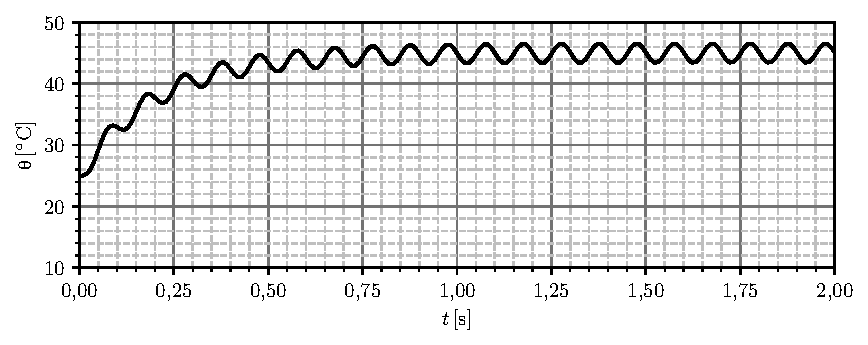
\includegraphics{fig/temperatura.pdf}
\caption{График температуре отпорника у зависности од времена}
\label{fig:\ID.}
\end{figure}

(б) У устаљеном режиму, сматрамо да је $\ee^{-at} \to 0$, док преостаје простопериодична компонента, тако да је 
устаљени одзив посматраног система дат као 
\begin{equation}
    \Delta\uptheta_{\rm ss}(t) =  20^\circ\rm C( 1 - 8\% \sin(2\upomega_0 t + \uppsi) ).
\end{equation}
па је амплитуда ове варијације једнака $\uptheta_{\rm m} = 20^\circ\rm C \cdot 8\% = 1,6^\circ\rm C$. 

